% =============================================================================
%  SSAH SST Optical Data Processing Pipeline — Technical Reference Manual
%  Build:  latexmk -pdf SSAH_SST_Pipeline_Manual.tex
% =============================================================================
\documentclass[11pt,a4paper]{article}

% ---- document control (edit here) -------------------------------------------
\newcommand{\doctitle}{SSAH SST Optical Data Processing Pipeline}
\newcommand{\docsubtitle}{Technical Reference Manual}
\newcommand{\docversion}{2.0}
\newcommand{\softversion}{2.0.0}
\newcommand{\docdate}{November 2026}
\newcommand{\docauthor}{Javed Iqbal}
\newcommand{\docorg}{Sharjah Astronomical Observatory (SSAH)}
\newcommand{\docstatus}{Public}
\newcommand{\doclicense}{BSD 3-Clause License}
\newcommand{\docrepo}{https://github.com/YOUR-GITHUB-USER/ssah-sst-pipeline}

% ---- packages ----------------------------------------------------------------
\usepackage[T1]{fontenc}
\usepackage[utf8]{inputenc}
\usepackage{charter}
\usepackage[scaled=0.92]{helvet}
\renewcommand{\ttdefault}{pcr}
\usepackage{amsmath,amssymb}
\usepackage[a4paper,margin=25mm,headheight=14pt]{geometry}
\usepackage{microtype}
\usepackage{xcolor,graphicx,tikz}
\usetikzlibrary{positioning,arrows.meta,fit,backgrounds}
\usepackage{booktabs,tabularx,longtable,array,multirow}
\usepackage{enumitem}
\usepackage{titlesec}
\usepackage{fancyhdr,lastpage}
\usepackage{caption}
\usepackage[most]{tcolorbox}
\usepackage{listings}
\usepackage[hidelinks]{hyperref}
\usepackage{etoolbox}
\usepackage{float}
\usepackage{needspace}

\definecolor{navy}{HTML}{1B3A6B}
\definecolor{teal}{HTML}{1E6B6B}
\definecolor{lgrey}{HTML}{F2F4F7}
\definecolor{mgrey}{HTML}{8A94A6}

\hypersetup{colorlinks=true,linkcolor=navy,urlcolor=teal,citecolor=teal,
  pdftitle={\doctitle\ -- \docsubtitle},pdfauthor={\docauthor},
  pdfsubject={Optical space surveillance and tracking data processing}}

\setlength{\parindent}{0pt}
\setlength{\parskip}{6pt plus 2pt}
\setlist{itemsep=2pt,topsep=4pt}
\renewcommand{\arraystretch}{1.25}
\captionsetup{font=small,labelfont={bf,color=navy},skip=6pt}

\titleformat{\section}{\sffamily\Large\bfseries\color{navy}}{\thesection}{0.8em}{}[\vspace{-4pt}{\color{navy}\titlerule[0.8pt]}]
\titleformat{\subsection}{\sffamily\large\bfseries\color{navy}}{\thesubsection}{0.7em}{}
\titleformat{\subsubsection}{\sffamily\normalsize\bfseries\color{teal}}{\thesubsubsection}{0.6em}{}
\titlespacing*{\section}{0pt}{18pt}{10pt}

\pagestyle{fancy}
\fancyhf{}
\fancyhead[L]{\sffamily\small\color{mgrey}\doctitle}
\fancyhead[R]{\sffamily\small\color{mgrey}\docsubtitle\ \textbullet\ v\docversion}
\fancyfoot[L]{\sffamily\small\color{mgrey}\docorg}
\fancyfoot[R]{\sffamily\small\color{mgrey}Page \thepage\ of \pageref*{LastPage}}
\renewcommand{\headrulewidth}{0.4pt}
\renewcommand{\headrule}{{\color{mgrey!50}\hrule width\headwidth height\headrulewidth}}

\lstset{basicstyle=\ttfamily\small,backgroundcolor=\color{lgrey},frame=single,
  rulecolor=\color{mgrey!40},framesep=6pt,xleftmargin=6pt,xrightmargin=6pt,
  columns=fullflexible,keepspaces=true,showstringspaces=false,breaklines=true,
  commentstyle=\color{teal},aboveskip=8pt,belowskip=8pt}

\newtcolorbox{keybox}[1][]{enhanced,colback=lgrey,colframe=navy,boxrule=0.6pt,
  arc=2pt,left=8pt,right=8pt,top=6pt,bottom=6pt,fonttitle=\sffamily\bfseries,
  coltitle=white,colbacktitle=navy,#1}
\newtcolorbox{notebox}{enhanced,colback=white,colframe=teal,boxrule=0.5pt,
  leftrule=3pt,arc=0pt,left=8pt,right=8pt,top=4pt,bottom=4pt}

% identifiers may break after "_", "." and "/" so long names fit table cells
\newcommand{\brkus}{\textunderscore\allowbreak}
\newcommand{\code}[1]{{\ttfamily\let\_\brkus #1}}
\newcommand{\cfg}[1]{{\ttfamily\small\let\_\brkus #1}}
\newcolumntype{P}[1]{>{\raggedright\arraybackslash}p{#1}}
\newcolumntype{L}{>{\raggedright\arraybackslash}X}

% =============================================================================
\begin{document}

% ---- title page ----------------------------------------------------------------
\begin{titlepage}
\thispagestyle{empty}
\begin{tikzpicture}[remember picture,overlay]
  \fill[navy] (current page.north west) rectangle ([yshift=-95mm]current page.north east);
  \fill[teal] ([yshift=-95mm]current page.north west) rectangle ([yshift=-98mm]current page.north east);
  \node[anchor=north west,text=white,font=\sffamily\small,inner sep=0pt]
     at ([xshift=25mm,yshift=-22mm]current page.north west)
     {\MakeUppercase{\docorg}};
  \node[anchor=north west,text=white,font=\sffamily\bfseries\fontsize{26}{31}\selectfont,
        text width=160mm,align=left,inner sep=0pt]
     at ([xshift=25mm,yshift=-38mm]current page.north west) {\doctitle};
  \node[anchor=north west,text=white!85!navy,font=\sffamily\Large,inner sep=0pt]
     at ([xshift=25mm,yshift=-74mm]current page.north west) {\docsubtitle};
  % decorative trail
  \foreach \i in {0,...,40}{
    \fill[white,opacity=0.10+0.015*\i] ([xshift=118mm+1.7mm*\i,yshift=-58mm-0.55mm*\i]current page.north west) circle (0.55mm);}
\end{tikzpicture}

\vspace*{95mm}
{\sffamily
\renewcommand{\arraystretch}{1.9}
\newcommand{\tplabel}[1]{\textcolor{mgrey}{\small #1}}
\begin{tabular}{@{}p{38mm}l@{}}
\tplabel{Software version} & {\large \softversion} \\
\tplabel{Document version} & {\large \docversion} \\
\tplabel{Date}             & {\large \docdate} \\
\tplabel{Author}           & {\large \docauthor} \\
\tplabel{Organisation}     & {\large \docorg} \\
\tplabel{Classification}   & {\large \docstatus} \\
\tplabel{License}          & {\large \doclicense} \\
\end{tabular}}
\renewcommand{\arraystretch}{1.25}

\vfill
{\sffamily\small\color{mgrey}
This manual describes the design, scientific conventions, configuration and
validation of a Python pipeline that converts raw optical FITS observations into
quality-controlled, star-referenced astrometry and photometry of resident space
objects, linked tracklets, TLE correlations, and CCSDS TDM / ADES data products.}

\vspace{6mm}
{\color{navy}\rule{\textwidth}{0.8pt}}
\end{titlepage}

% ---- document control ----------------------------------------------------------------
\section*{Document Control}
\addcontentsline{toc}{section}{Document Control}

\begin{tabularx}{\textwidth}{@{}>{\bfseries}p{40mm}L@{}}
\toprule
Title & \doctitle\ --- \docsubtitle \\
Software & \code{ssah-sst-pipeline} \softversion{} (Python $\geq$ 3.10) \\
Author & \docauthor, \docorg \\
Classification & \docstatus \\
License & \doclicense{} (software and this manual) \\
Repository & {\small\url{\docrepo}} \\
Source & \code{docs/\allowbreak manual/\allowbreak SSAH\_SST\_Pipeline\_Manual.\allowbreak tex} in the repository \\
\bottomrule
\end{tabularx}

\subsection*{Revision history}
\begin{tabularx}{\textwidth}{@{}p{16mm}p{30mm}L@{}}
\toprule
\textbf{Version} & \textbf{Date} & \textbf{Changes} \\
\midrule
1.0 & June 2026 & Initial internal release (software 1.0.0). \\
2.0 & November 2026 & First public release. Complete revision for software 2.0.0. Corrected TLE propagation chain, mid-exposure
epochs, segmentation-based trail measurement, kinematic tracklet linking, verified astrometry against a
local Gaia DR3 store, CCSDS TDM output, extended QC dimensions, validation chapter.
Online plate solving and live TLE retrieval removed (offline operation). \\
\bottomrule
\end{tabularx}

\vspace{8mm}
\begingroup
\hypersetup{linkcolor=black}
\renewcommand{\contentsname}{\sffamily\color{navy}Contents}
\setcounter{tocdepth}{2}
\setlength{\parskip}{0pt}
\tableofcontents
\endgroup
\clearpage

% =============================================================================
\section{Overview}

The pipeline post-processes optical observations of resident space objects (RSOs) taken
at the Sharjah Astronomical Observatory. Starting from raw FITS frames it produces:

\begin{itemize}
  \item a per-frame quality-control (QC) matrix with independent photometric and astrometric decisions;
  \item calibrated, star-referenced RSO positions at the correct mid-exposure epochs, with uncertainties;
  \item calibrated magnitudes in the reference-catalogue band;
  \item tracklets linking each object across frames, correlated with a TLE catalogue, and
        uncorrelated tracks (UCTs) for objects that match no catalogued orbit;
  \item exchange files in CCSDS Tracking Data Message (TDM) and IAU ADES format.
\end{itemize}

\subsection{Design principles}

\begin{description}[style=nextline,leftmargin=0pt,font=\sffamily\bfseries\color{navy}]
\item[Two quality tracks]
Astrometry and photometry tolerate different defects. A trailed, partly saturated or
low-SNR frame may be useless for brightness but still yield a valid centroid. Every frame
receives two independent decisions, \code{photometry\_pass} and \code{astrometry\_pass}.
\item[Verified astrometry only]
A WCS written by the mount's pointing model is typically tens of arcseconds to arcminutes
in error. Positions are reported only from frames whose plate solution has been verified
and refitted against reference stars.
\item[Correct epochs]
Every measurement is time-stamped at the mid-exposure of the pixels it was measured on,
including clock bias and rolling-shutter delays. For low-Earth-orbit objects, timing is
usually the dominant error source.
\item[Offline by design]
Reference stars come from a local Gaia DR3 store built in advance and TLEs from a local
file. No step depends on an external service at run time.
\item[Configuration, not code]
Every threshold and instrument parameter is in one YAML file. A site file contains only
the values that differ from the defaults.
\item[Batch safety]
A corrupt or anomalous frame is recorded as a QC failure with its reason; it never stops
a run.
\end{description}

\subsection{Key characteristics}

\begin{table}[H]
\centering\small
\begin{tabularx}{\textwidth}{@{}P{48mm}L@{}}
\toprule
\textbf{Property} & \textbf{Detail} \\
\midrule
Processing mode & Post-processing of an observing session, offline \\
Tracking modes & Sidereal (stars are points, RSOs trail) and target-rate (RSO is a point, stars trail) \\
Quality control & Twelve criteria, two independent decisions per frame \\
Astrometric reference & Gaia DR3, proper motions applied to the observation epoch \\
Epochs & Mid-exposure UTC, time bias and rolling shutter, microsecond output \\
Known-object correlation & SGP4 with light-time and star-referenced convention; along/cross-track O$-$C \\
Exchange formats & CCSDS TDM (KVN, RADEC); ADES PSV \\
Validation & 78 automated tests, end-to-end run on synthetic data with ground truth,
             SGP4 cross-check against skyfield \\
Requirements & Python $\geq$ 3.10; astropy, sep, photutils, sgp4, astroscrappy, numpy, scipy, pandas \\
\bottomrule
\end{tabularx}
\caption{Pipeline key characteristics.}
\end{table}

% =============================================================================
\section{Installation and Quick Start}

\subsection{Installation}
\noindent\begin{minipage}{\linewidth}
\begin{lstlisting}
git clone https://github.com/YOUR-GITHUB-USER/ssah-sst-pipeline
cd ssah-sst-pipeline
pip install -e ".[all]"     # pipeline, online catalogue tools, tests
pytest                      # 78 tests, about 40 s
\end{lstlisting}
\end{minipage}\par
The optional extra \code{online} installs \code{astroquery}, needed only to download
reference stars. The astrometry.net \code{solve-field} program is optional and used only
for frames without a WCS in the header.

\subsection{Command-line tools}
\begin{table}[H]
\centering\small
\begin{tabularx}{\textwidth}{@{}p{30mm}L@{}}
\toprule
\textbf{Command} & \textbf{Purpose} \\
\midrule
\code{sst-pipeline} & Process a folder of FITS frames (Section~\ref{sec:stages}). \\
\code{sst-refcat}   & Build or extend the local Gaia DR3 reference store (Section~\ref{sec:refcat}). \\
\code{sst-tle}      & Download a TLE catalogue from CelesTrak for offline use. \\
\code{sst-synthetic}& Generate a synthetic sequence with ground truth. \\
\code{sst-demo}     & Generate, process and compare against truth in one step. \\
\bottomrule
\end{tabularx}
\caption{Console commands installed with the package.}
\end{table}

\subsection{First run}
\noindent\begin{minipage}{\linewidth}
\begin{lstlisting}
sst-demo                     # synthetic end-to-end check

cp config/site_template.yaml config/ssah_site.yaml
#   ... fill in every [REQUIRED] value ...
sst-refcat --geo-belt        # once, on a networked machine
sst-tle --group active --out data/tle_catalog.txt
sst-pipeline /data/night1 /results/night1 \
    --config config/ssah_site.yaml
\end{lstlisting}
\end{minipage}\par

% =============================================================================
\section{Processing Stages}\label{sec:stages}

Stages 1--8 run for every frame; stages 9--12 run once per session, because they need all
frames.

\begin{figure}[H]
\centering
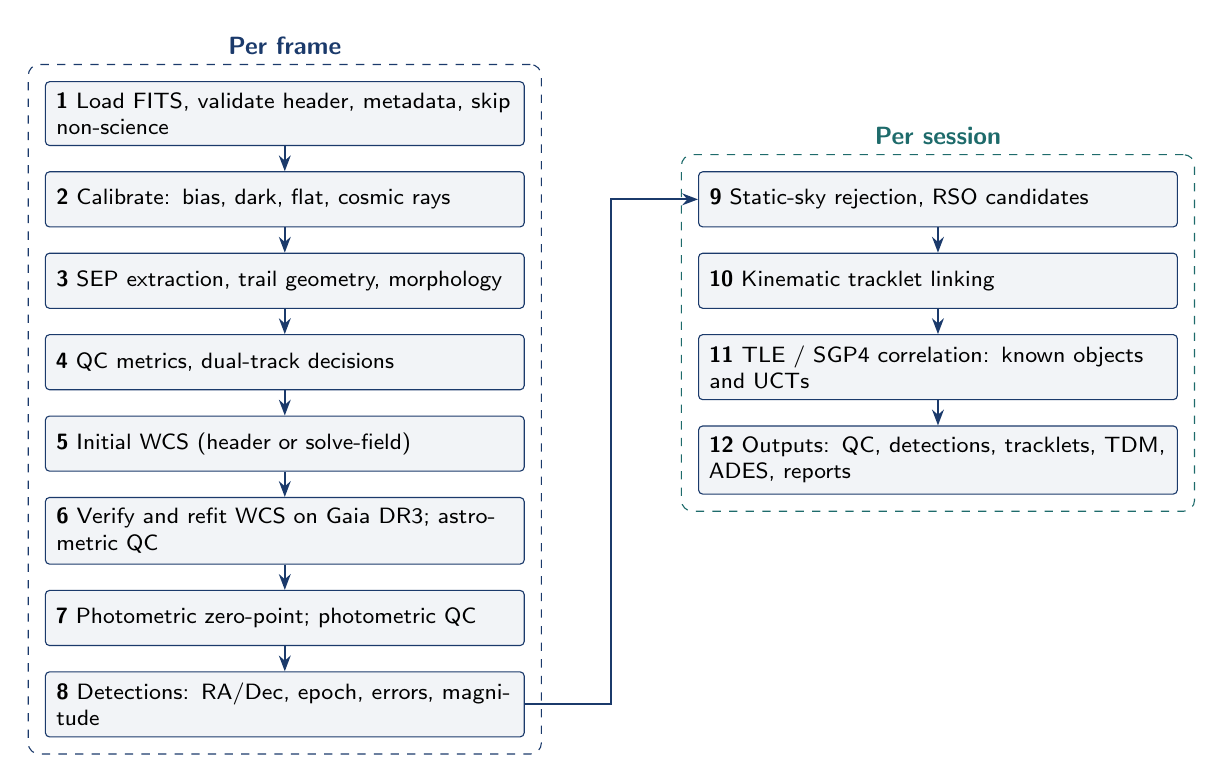
\begin{tikzpicture}[node distance=3.2mm,
  box/.style={draw=navy,fill=lgrey,rounded corners=1.5pt,font=\sffamily\footnotesize,
              text width=58mm,align=left,inner sep=4pt,minimum height=7mm},
  arr/.style={-{Stealth[length=2mm]},navy,thick}]
\node[box] (a) {\textbf{1} Load FITS, validate header, metadata, skip non-science};
\node[box,below=of a] (b) {\textbf{2} Calibrate: bias, dark, flat, cosmic rays};
\node[box,below=of b] (c) {\textbf{3} SEP extraction, trail geometry, morphology};
\node[box,below=of c] (d) {\textbf{4} QC metrics, dual-track decisions};
\node[box,below=of d] (e) {\textbf{5} Initial WCS (header or solve-field)};
\node[box,below=of e] (f) {\textbf{6} Verify and refit WCS on Gaia DR3; astrometric QC};
\node[box,below=of f] (g) {\textbf{7} Photometric zero-point; photometric QC};
\node[box,below=of g] (h) {\textbf{8} Detections: RA/Dec, epoch, errors, magnitude};
\begin{scope}[on background layer]
\node[draw=navy,dashed,rounded corners,fit=(a)(h),inner sep=6pt,label={[font=\sffamily\small\bfseries,text=navy]above:Per frame}] (pf) {};
\end{scope}
\node[box,right=22mm of b] (i) {\textbf{9} Static-sky rejection, RSO candidates};
\node[box,below=of i] (j) {\textbf{10} Kinematic tracklet linking};
\node[box,below=of j] (k) {\textbf{11} TLE / SGP4 correlation: known objects and UCTs};
\node[box,below=of k] (l) {\textbf{12} Outputs: QC, detections, tracklets, TDM, ADES, reports};
\begin{scope}[on background layer]
\node[draw=teal,dashed,rounded corners,fit=(i)(l),inner sep=6pt,label={[font=\sffamily\small\bfseries,text=teal]above:Per session}] (ps) {};
\end{scope}
\foreach \x/\y in {a/b,b/c,c/d,d/e,e/f,f/g,g/h,i/j,j/k,k/l} \draw[arr] (\x) -- (\y);
\draw[arr] (h.east) -| ([xshift=-11mm]i.west) -- (i.west);
\end{tikzpicture}
\caption{Processing flow. A frame failing the astrometry track after stage 4 or 6 produces no detections.}
\end{figure}

\begin{table}[H]
\centering\small
\begin{tabularx}{\textwidth}{@{}p{8mm}P{55mm}L@{}}
\toprule
\textbf{\#} & \textbf{Module} & \textbf{Function} \\
\midrule
1  & \code{io/\allowbreak fits\_loader}, \code{io/\allowbreak header\_validator}, \code{io/\allowbreak metadata\_extractor} & Load frames (incl.\ compressed and multi-extension), validate headers, extract metadata; skip bias/dark/flat frames by \code{IMAGETYP}. \\
2  & \code{calibration/\allowbreak calibration\_manager} & Bias, scaled dark and flat correction; L.A.Cosmic cleaning. \\
3  & \code{detection/\allowbreak source\_extractor}, \code{detection/\allowbreak source\_classifier} & One SEP pass; moment and profile trail geometry; fragment merging; POINT / TRAILED / ARTIFACT / EXTENDED. \\
4  & \code{qc/\allowbreak metrics}, \code{qc/\allowbreak qc\_matrix} & Image-quality metrics and dual-track decisions. \\
5--6 & \code{astrometry/\allowbreak wcs\_solver}, \code{astrometry/\allowbreak reference\_catalog}, \code{astrometry/\allowbreak catalog\_store} & Initial WCS; offset vote, one-to-one match and TAN+SIP refit against Gaia DR3. \\
7  & \code{photometry/\allowbreak aperture\_photometry} & Zero-point from the same reference stars; CCD-equation errors. \\
8  & \code{astrometry/\allowbreak position\_extractor} & Sky position, mid-exposure epoch, uncertainty, magnitude. \\
9--10 & \code{tracking/\allowbreak linker} & Static-sky test, candidate selection, constant-rate linking. \\
11 & \code{tracking/\allowbreak tle\_manager}, \code{tracking/\allowbreak orbit\_propagator}, \code{tracking/\allowbreak known\_object\_matcher} & SGP4 prediction and correlation. \\
12 & \code{output/\allowbreak writers}, \code{reporting/\allowbreak report\_generator} & Data products, workbook, plots. \\
\bottomrule
\end{tabularx}
\caption{Stages and modules.}
\end{table}

% =============================================================================
\section{Configuration}

The packaged file \code{sst\_pipeline/\allowbreak defaults.\allowbreak yaml} holds every parameter with comments.
A site file (copied from \code{config/\allowbreak site\_template.\allowbreak yaml}) is deep-merged over it, so it
contains only site-specific values. Keys that do not exist in the defaults trigger a
warning, so a misspelled parameter is not silently ignored.

\begin{table}[H]
\centering\small
\begin{tabularx}{\textwidth}{@{}P{60mm}L@{}}
\toprule
\textbf{Parameter} & \textbf{How to obtain} \\
\midrule
\cfg{instrument.\allowbreak gain\_e\_per\_adu} & Camera datasheet or photon-transfer curve. \\
\cfg{instrument.\allowbreak read\_noise\_e} & Camera datasheet, or bias-frame statistics. \\
\cfg{instrument.\allowbreak saturation\_adu} & The non-linearity limit, not the ADC maximum. \\
\cfg{instrument.\allowbreak pixel\_scale\_arcsec} & $206265\times$ pixel size / focal length; confirmed by plate solutions. \\
\cfg{site.\allowbreak latitude\_deg}, \cfg{longitude\_deg}, \cfg{height\_m} & Surveyed geodetic coordinates. \\
\cfg{site.\allowbreak iau\_obs\_code} & MPC observatory code, if assigned (ADES only). \\
\cfg{observation.\allowbreak tracking\_mode} & \code{sidereal} or \code{rate}. \\
\cfg{timing\_calibration.\allowbreak date\_obs\_reference} & Whether the camera software writes exposure start, mid or end. \\
\cfg{timing\_calibration.\allowbreak time\_bias\_ms} & Measured on sky (Section~\ref{sec:timing}). \\
\cfg{timing\_calibration.\allowbreak shutter\_type}, \cfg{readout\_time\_ms} & \code{global}, or \code{rolling} with readout time (CMOS). \\
\cfg{calibration.\allowbreak master\_*\_path} & Master bias (ADU); dark bias-subtracted per second; flat normalised, same filter. \\
\cfg{astrometry.\allowbreak reference\_catalog\_dir} & Local Gaia DR3 store (Section~\ref{sec:refcat}). \\
\cfg{tle\_tracking.\allowbreak tle\_file\_path} & TLE file from \code{sst-tle}; refresh daily for LEO. \\
\bottomrule
\end{tabularx}
\caption{Site parameters to set before processing real data.}
\end{table}

% =============================================================================
\section{FITS Header Validation}

Keyword rules are declared in the configuration. A missing or unparsable mandatory keyword
fails both QC tracks; optional keywords produce warnings.

\begin{table}[H]
\centering\small
\begin{tabularx}{\textwidth}{@{}P{24mm}P{38mm}L@{}}
\toprule
\textbf{Keyword} & \textbf{Aliases} & \textbf{Type and purpose} \\
\midrule
\multicolumn{3}{@{}l}{\textit{Mandatory}} \\
\code{DATE-OBS} & --- & ISO-8601 UTC; date-only values are combined with \code{TIME-OBS} / \code{UT}. Epoch of every measurement. \\
\code{EXPTIME}  & \code{EXPOSURE} & 0.0001--600 s. Mid-exposure epoch, rates, fluxes. \\
\code{OBJECT}   & \code{TARGET} & Links the frame to the observing plan. \\
\code{TELESCOP} & \code{TELESCOPE} & Instrument traceability. \\
\code{INSTRUME} & \code{INSTRUMENT}, \code{CAMERA} & Camera identification, calibration matching. \\
\midrule
\multicolumn{3}{@{}l}{\textit{Recommended}} \\
\code{RA}, \code{DEC} & \code{OBJCTRA}, \code{OBJCTDEC} & Degrees or sexagesimal strings (``\code{10 00 00.\allowbreak 0}''). Plate-solve hint. \\
WCS keywords & \code{CTYPEi}, \code{CRVALi}, \code{CRPIXi}, \code{CD}/\code{CDELT} & Initial plate solution (verified before use). \\
\code{IMAGETYP} & \code{IMGTYPE}, \code{FRAMETYP} & Non-science frames (bias, dark, flat) are skipped. \\
\code{AIRMASS}, \code{FILTER}, \code{CCD-TEMP}, \code{OBSERVER} & --- & Recorded; airmass is computed from site and pointing when absent. \\
\bottomrule
\end{tabularx}
\caption{Header keywords.}
\end{table}

% =============================================================================
\section{Calibration}

Science frames are reduced as
\begin{equation}
I_\mathrm{cal} = \frac{I_\mathrm{raw} - B - D_{1\,\mathrm{s}}\, t_\mathrm{exp}}{F},
\end{equation}
where $B$ is the master bias, $D_{1\,\mathrm{s}}$ the bias-subtracted dark per second and $F$
the normalised flat. Masters whose shape differs from the frame are rejected and logged.
Cosmic rays are removed with L.A.Cosmic \cite{vandokkum2001} (astroscrappy). The
cosmic-ray mask is kept for QC. Saturation and hot pixels are measured on the raw frame,
because calibration moves pixels away from the detector ceiling.

% =============================================================================
\section{Source Extraction and Trail Measurement}

A single SEP \cite{bertin1996,barbary2016} extraction per frame serves QC, plate verification,
photometric calibration and target measurement. Each source is re-measured from its
segmentation pixels with flux-weighted second moments $\lambda_1 \geq \lambda_2$ along and
across its principal axis. For a uniform trail of length $L$ convolved with a PSF of width
$\sigma$:
\begin{equation}
\lambda_1 = \frac{L^2}{12} + \sigma^2,\qquad \lambda_2 = \sigma^2
\quad\Rightarrow\quad L = \sqrt{12\,(\lambda_1-\lambda_2)} .
\end{equation}

\textbf{Profile refinement.} Moments are biased when a trail crosses a star or is split by
deblending. The along-track profile within $\pm 2.5\sigma$ of the axis,
\begin{equation}
P(s) = P_0\left[\Phi\!\left(\tfrac{L/2 - s}{\sigma}\right) - \Phi\!\left(\tfrac{-L/2 - s}{\sigma}\right)\right],
\end{equation}
falls to exactly half its plateau $P_0$ at the true end points $s=\pm L/2$. The pipeline
re-fits the axis from across-track centroids, median-filters $P(s)$, and takes the
half-maximum crossings as end points. The midpoint is the mid-exposure position, and
$P_0 L$ gives a flux that is robust to crossing stars. Collinear fragments of one trail are
merged before this step.

\textbf{Classification.} \code{TRAILED}: elongation $\geq 2.5$ and $L\geq 8$\,px.
\code{ARTIFACT}: sharper than the PSF (hot pixel, cosmic ray), or saturated and aligned with a
detector axis (charge bleeding). \code{EXTENDED}: FWHM above 15\,px. Otherwise \code{POINT}.
The role of each class depends on the tracking mode:

\begin{table}[H]
\centering\small
\begin{tabular}{@{}lccc@{}}
\toprule
\textbf{Tracking mode} & \textbf{Stars appear} & \textbf{RSOs appear} & \textbf{Reference stars for WCS / ZP} \\
\midrule
\code{sidereal} & POINT & TRAILED & POINT sources \\
\code{rate}     & TRAILED & POINT & TRAILED sources (midpoints) \\
\bottomrule
\end{tabular}
\caption{Morphology roles.}
\end{table}

% =============================================================================
\section{Quality Control}

Each frame receives two decisions. Thresholds are the defaults in \code{defaults.\allowbreak yaml};
calibrate them on real SSAH data.

\begin{table}[H]
\centering\small
\begin{tabularx}{\textwidth}{@{}p{35mm}p{30mm}LL@{}}
\toprule
\textbf{Metric} & \textbf{Measured on} & \textbf{Photometry track} & \textbf{Astrometry track} \\
\midrule
Header validity & header & fail if invalid & fail if invalid \\
Signal presence & SEP catalogue & $\geq 1$ source & $\geq 1$ source \\
SNR (unsaturated) & SEP catalogue & $\geq 10$ & $\geq 5$ \\
Saturated pixels & raw frame & $\leq 0.05\%$ & $\leq 2\%$ \\
Seeing (FWHM) & reference stars & $\leq 6''$ & $\leq 10''$ \\
Star ellipticity & reference stars (sidereal) & $\leq 0.35$ (tracking/focus) & --- \\
Background stability & rolling window & level and noise within $4\sigma$ & --- \\
Transparency & star count & $\geq 50\%$ of sequence median & --- \\
Artefacts & raw / calibrated & CR $\leq 0.2\%$, hot px, columns, gradient & CR $\leq 1\%$ \\
Trail length & SEP catalogue & $\leq 2000$\,px & --- \\
Plate solution & Gaia DR3 fit & --- & verified; RMS $\leq 1.5''$ \\
Zero-point scatter & Gaia DR3 stars & $\geq 5$ stars; RMS $\leq 0.10$ mag & --- \\
\bottomrule
\end{tabularx}
\caption{QC metrics and default thresholds.}
\end{table}

Background stability and transparency are judged against a rolling window of the last ten
valid frames (at least five), using robust statistics:
$|x - \tilde{x}| / \max(1.4826\,\mathrm{MAD},\,0.02\,\tilde{x}) \leq 4$.

% =============================================================================
\section{Astrometry}

\subsection{Reference catalogue}\label{sec:refcat}
Reference stars are Gaia DR3 \cite{gaia2023} sources (G\,$<$\,16 by default) stored locally in
cells of about $2^\circ\times2^\circ$. Each cell is one compressed file with position (ICRS,
epoch J2016.0), proper motion and G magnitude. At run time only the cells covering a
frame are read, and positions are propagated to the observation epoch:
\begin{equation}
\alpha(t) = \alpha_0 + \frac{\mu_{\alpha*}}{\cos\delta_0}(t - 2016.0),\qquad
\delta(t) = \delta_0 + \mu_\delta (t - 2016.0).
\end{equation}

The store is built in advance with \code{sst-refcat}, which is resumable and downloads
from VizieR (CDS, then the CfA mirror) with the ESA Gaia archive as fallback, each under a
timeout:

\noindent\begin{minipage}{\linewidth}
\begin{lstlisting}
sst-refcat --geo-belt --dry-run        # preview the cells
sst-refcat --geo-belt                  # GEO band seen from the site
sst-refcat --geo-belt --margin 15      # + inclined GEO objects
sst-refcat --site-visible              # sky above 20 deg altitude
sst-refcat --around 150 20 1.5         # one field
sst-refcat --from-csv gaia_export.csv  # import, no download
\end{lstlisting}
\end{minipage}\par

From SSAH (latitude $25.36^\circ$\,N, altitude $>20^\circ$) the geostationary ring appears
near declination $-4^\circ$ because of parallax. At G\,$<$\,16 the GEO belt needs 719 cells,
the belt $\pm15^\circ$ 2\,843 cells, and the whole visible sky 8\,985 cells. When
\code{sst-pipeline} runs with \code{--catalog}, cells missing for an observed field are
downloaded once and kept.

\subsection{Plate verification and refit}
\begin{enumerate}
\item The initial WCS comes from the header or, with \code{--solve-wcs}, from a local
      astrometry.net \cite{lang2010} solve of the calibrated frame with scale and position hints.
\item Reference stars are projected with the initial WCS. A two-dimensional vote over all
      star--catalogue pixel offsets (search radius $120''$) absorbs pointing errors.
\item Stars are matched one-to-one within $2''$, and a TAN projection is fitted
      (with SIP distortion of order 2 when at least 15 stars match), with iterative
      $3\sigma$ clipping.
\item The plate is \emph{verified} when at least 8 stars match. Its RMS,
\begin{equation}
\mathrm{RMS}_\mathrm{astro} = \sqrt{\left\langle (\Delta\alpha\cos\delta)^2 + (\Delta\delta)^2\right\rangle},
\end{equation}
      must not exceed $1.5''$.
\end{enumerate}

\subsection{Positions and uncertainties}
Each detection's centroid uncertainty is its RMS width divided by its SNR along each
principal axis, rotated to RA/Dec through the local WCS. It is added in quadrature to the
plate RMS of the corresponding axis. Pixel coordinates are 0-based, consistent with astropy.

% =============================================================================
\section{Photometry}

Point sources use a circular aperture of radius $1.5\times$FWHM with a sigma-clipped
annulus ($4$--$7\times$FWHM). Trails use a rotated rectangle of length $L+3\,$FWHM and half-width
$1.5\,$FWHM with a rectangular sky annulus, as in trailed-source photometry \cite{veres2012}. Both are corrected to total flux with the Gaussian
enclosed-energy fraction ($1-e^{-r^2/2\sigma^2}$ for a circle, $\mathrm{erf}(h/\sqrt2\sigma)$ times
the along-track fraction for a trail). If stars inside a trail aperture inflate the flux, the
profile flux $P_0L$ is used instead.

The uncertainty follows the CCD equation \cite{merline1995}:
\begin{equation}
\sigma_F^2 = \frac{F}{g} + n_\mathrm{ap}\,\sigma_s^2 + \frac{n_\mathrm{ap}^2\,\sigma_s^2}{n_\mathrm{sky}}
\qquad[\mathrm{ADU}^2],
\end{equation}
with gain $g$ (e$^-$/ADU) and empirical sky noise $\sigma_s$ per pixel.

Instrumental magnitudes are $m_\mathrm{inst} = -2.5\log_{10}(F/t_\mathrm{exp})$. The frame
zero-point is the median of $m_\mathrm{cat} - m_\mathrm{inst}$ over unsaturated reference stars
with SNR\,$\geq20$, with MAD-based clipping. The photometric RMS is the scatter of the retained
residuals. A frame zero-point already includes atmospheric extinction, so
$m = m_\mathrm{inst} + \mathrm{ZP}$. Only when no zero-point can be measured is the configured
fallback used, $m = m_\mathrm{inst} + \mathrm{ZP}_0 - kX$. Magnitudes from it are flagged as
uncalibrated and are not exported.

% =============================================================================
\section{Timing}\label{sec:timing}

The epoch of a measurement at detector row $y$ is
\begin{equation}
t = t_\mathrm{DATE\text{-}OBS} - \Delta_\mathrm{ref} + t_\mathrm{bias} + \frac{y}{N}\,T_\mathrm{readout} + \frac{t_\mathrm{exp}}{2},
\qquad \Delta_\mathrm{ref}\in\{0,\ t_\mathrm{exp}/2,\ t_\mathrm{exp}\},
\end{equation}
where $\Delta_\mathrm{ref}$ depends on whether DATE-OBS marks the start, middle or end of the
exposure. The row term applies only to rolling shutters (\code{readout\_time\_ms} over $N$
rows). For uniform motion the flux-weighted trail centroid lies at the mid-exposure position, so
the same epoch applies to point sources and trail midpoints. Epochs are written with
microsecond resolution.

A timing error $\delta t$ displaces an object moving at angular rate $\omega$ by
\begin{equation}
\delta\theta = \omega\,\delta t .
\end{equation}

\begin{table}[H]
\centering\small
\begin{tabular}{@{}lccc@{}}
\toprule
\textbf{Object} & \textbf{Rate $\omega$} & \textbf{10 ms error} & \textbf{Half of a 2 s exposure} \\
\midrule
LEO near zenith (e.g.\ ISS) & $\approx1^\circ$/s & $\approx36''$ & $\approx1^\circ$ \\
GEO, sidereal tracking & $15''$/s & $0.15''$ & $15''$ \\
\bottomrule
\end{tabular}
\caption{Effect of timing errors on position.}
\end{table}

\begin{notebox}
\textbf{Calibrating the time bias.} Observe GNSS satellites (GPS, Galileo), whose orbits are
known to centimetre level, and process them with a TLE or precise ephemeris. The pipeline
reports for each identified tracklet the mean along-track O$-$C divided by the predicted rate
(\code{along\_track\_time\_offset\_s}). Averaged over several satellites, this is the clock and
shutter bias to enter as \code{time\_bias\_ms}.
\end{notebox}

% =============================================================================
\section{Tracklets and Uncorrelated Tracks}

\textbf{Static sky.} A detection whose sky position recurs within $3''$ in at least three frames
is fixed on the sky (a star or galaxy below the catalogue limit) and is rejected.

\textbf{Candidates.} RSO candidates are detections that are not catalogue stars, not static,
not artefacts, and have the morphology expected for the tracking mode. In sidereal mode, point
sources become candidates only when the static test is possible (at least three frames).

\textbf{Linking.} Pairs of candidates in different frames within 120\,s whose implied rate lies
between $0.2$ and $4000''$/s seed a constant-rate model in the tangent plane. For trails, the
motion direction and rate must also agree with the trail axis ($\pm10^\circ$) and the trail
rate ($\pm30\%$). Each seed is grown by adding the nearest candidate within $6''$ of the
prediction in every later frame. The longest chain with at least three positions and a fit RMS
$\leq 3''$ becomes a tracklet. Unlinked trails are kept as single-frame tracklets; a single trail
gives a position and a rate, with direction ambiguous by $180^\circ$.

% =============================================================================
\section{Known-Object Identification}

\subsection{Prediction chain}
\begin{enumerate}
\item SGP4 \cite{vallado2006} with WGS-72 constants propagates every catalogue object at once to
      the measurement epoch, giving TEME position and velocity.
\item Light-time correction: $\mathbf{r}(t-\rho/c) \approx \mathbf{r} - \mathbf{v}\,\rho/c$
      (about 25\,m for LEO).
\item TEME is transformed to GCRS (astropy \cite{astropy2022}), and the site's GCRS position is subtracted to give
      the topocentric line of sight.
\item \textbf{Star-referenced convention.} The plate solution maps the apparent star field onto
      aberration-free catalogue positions, removing the annual aberration ($\approx20''$) that
      stars show. An Earth-orbiting object shows no annual aberration, so its measured position
      carries the opposite shift. The line-of-sight \emph{direction} is therefore transformed from
      GCRS to ICRS as a unit vector, which applies the same correction as the plate solution.
      Diurnal aberration affects stars and satellite alike and cancels.
\item Altitude and azimuth are computed from the Earth-fixed topocentric vector. The apparent
      rate and direction of motion come from predictions at $t\pm0.5$\,s.
\end{enumerate}

\subsection{Matching}
TLE errors are dominated by the along-track component \cite{flohrer2008}. The O$-$C offset is
therefore decomposed along and across the predicted direction of motion and tested against
separate tolerances.

\begin{table}[H]
\centering\small
\begin{tabularx}{\textwidth}{@{}p{55mm}L@{}}
\toprule
\textbf{Criterion} & \textbf{Default} \\
\midrule
Along-track $|$O$-$C$|$ & $\leq 900''$ \\
Cross-track $|$O$-$C$|$ & $\leq 180''$ \\
Trail rate vs predicted rate & within $\pm30\%$ \\
Trail axis vs predicted direction & within $15^\circ$ (modulo $180^\circ$) \\
Object altitude & above the horizon \\
Quality \code{GOOD} & inside the half-size tolerance ellipse and TLE age $\leq14$ days; otherwise \code{MARGINAL} \\
\bottomrule
\end{tabularx}
\caption{Correlation criteria.}
\end{table}

A tracklet takes the NORAD identity held by the majority of its detections, provided its fitted
rate agrees with the prediction. Tracklets without an identity are reported as uncorrelated
tracks (UCTs).

% =============================================================================
\section{Output Files}

\begin{table}[H]
\centering\small
\begin{tabularx}{\textwidth}{@{}P{48mm}L@{}}
\toprule
\textbf{File} & \textbf{Contents} \\
\midrule
\code{qc\_matrix.\allowbreak csv} & Per-frame metrics, WCS and zero-point statistics, both decisions with reasons. \\
\code{rejected\_frames.\allowbreak log} & Human-readable rejection reasons per track. \\
\code{session\_metadata.\allowbreak csv} & Parsed header values for every science frame. \\
\code{skipped\_frames.\allowbreak csv} & Non-science frames that were skipped. \\
\code{detections.\allowbreak csv} & Every non-star detection: epoch, RA/Dec and uncertainties, magnitude, morphology, status
  (\code{LINKED}, \code{SINGLE\_STREAK}, \code{UNLINKED}, \code{STATIC}), tracklet, NORAD ID, O$-$C. \\
\code{tracklets.\allowbreak csv} & One row per tracklet: rate, position angle, fit RMS, mean magnitude, identification,
  along/cross-track O$-$C, time offset. \\
\code{uncorrelated\_tracks.\allowbreak csv} & Tracklets not matched to the TLE catalogue. \\
\code{observations\_tdm.\allowbreak kvn} & CCSDS TDM \cite{ccsds2020}: \code{ANGLE\_TYPE = RADEC}, \code{REFERENCE\_FRAME = ICRF},
  UTC, one segment per tracklet, verified plates only. \\
\code{observations\_ades.\allowbreak psv} & ADES PSV for archiving. The MPC does not accept artificial-satellite observations. \\
\code{qc\_summary.\allowbreak json} & Session totals. \\
\code{SST\_QC\_Report.\allowbreak xlsx} & Summary, QC Matrix, Metadata, Tracklets, Detections sheets. \\
\code{plot\_01}--\code{plot\_05} & Pass rates, SNR, background, seeing and plate RMS, star counts. \\
\code{pipeline\_<UTC>.\allowbreak log} & Full session log. \\
\bottomrule
\end{tabularx}
\caption{Data products written per session.}
\end{table}

% =============================================================================
\section{Validation}

\subsection{Synthetic sequence with ground truth}
\code{sst-synthetic} renders a physically consistent sequence: twelve $1024^2$ frames at
$0.82''$/px, 2\,s exposures every 10\,s, Poisson and read noise, and a fixed star field
(catalogued and faint uncatalogued stars). It contains three moving objects and quality-control
test cases: cosmic rays, cloud, a saturated star with charge bleeding, a missing header
keyword, and a bias frame. The header WCS is deliberately offset by $29''$ and rotated by
$0.05^\circ$.

\begin{table}[H]
\centering\small
\begin{tabular}{@{}lccc@{}}
\toprule
& \textbf{Trailed RSO} & \textbf{Slow point RSO} & \textbf{Fast single streak} \\
\midrule
Detected as & 10-frame tracklet & 11-frame tracklet & single streak \\
Position error, median / max & $0.06''$ / $0.19''$ & $0.01''$ / $0.04''$ & $0.14''$ \\
Rate, recovered (true) & $6.001''$/s (6.0) & $0.600''$/s (0.6) & $149.99''$/s (150) \\
Position angle, recovered (true) & $59.96^\circ$ (60) & $200.02^\circ$ (200) & $115.00^\circ$ (115) \\
Magnitude, recovered (true) & 12.51 (12.5) & 13.00 (13.0) & 10.50 (10.5) \\
\bottomrule
\end{tabular}
\caption{Recovery of the synthetic objects.}
\end{table}

Plates were corrected by $29.2''$ to an RMS of $0.04''$. Zero-points agree with the injected
value to within 0.03\,mag. Epochs equal the true mid-exposure times. No star was reported as an
RSO. The quality-control outcomes were as designed: the bias frame was skipped, the frame with a
missing keyword failed both tracks, the cloud and bleeding-star frames failed photometry only,
and the cosmic-ray frame was cleaned and passed.

\subsection{Orbit prediction}
For an ISS pass at $43.6^\circ$ altitude, the geometric topocentric predictions agree with the
independent skyfield implementation to $1.4''$ in position, $0.0001^\circ$ in altitude and 1\,m
in range. A known along-track timing offset of 50\,ms is recovered by the time-offset estimate to
within 2\,ms.

\subsection{Test suite}
The 78 automated tests (\code{pytest}) cover timing, header parsing, calibration, extraction and
trail geometry (including trails crossing bright stars), photometric flux recovery and error
model, plate refit, catalogue-store geometry and download fallbacks (with simulated servers),
QC decisions, linking, SGP4 correlation and the end-to-end run above.

\begin{notebox}
This is a validation of logic and accuracy on synthetic data. Thresholds, the time bias, and
photometric performance must still be established on real SSAH observations.
\end{notebox}

% =============================================================================
\section{Limitations and Next Steps}

\begin{itemize}
\item \textbf{Instrument and site values} in the configuration are provisional until confirmed
      (gain, read noise, non-linearity limit, surveyed coordinates, DATE-OBS convention).
\item \textbf{Time bias} must be measured on sky before reporting LEO positions.
\item \textbf{Thresholds} are defaults and should be tuned on real noise statistics.
\item \textbf{Target-rate tracking} is unit-tested; an end-to-end check on real frames is pending.
\item \textbf{Live downloads} (VizieR, ESA, CelesTrak) have been exercised against simulated servers
      only; a first single-field build confirms the path (\code{sst-refcat --around}).
\item \textbf{Photometric band}: unfiltered frames are calibrated to Gaia G without a colour term;
      expect object-colour-dependent offsets of a few tenths of a magnitude.
\item \textbf{Orbit determination}, conjunction assessment and re-entry analysis are outside the
      scope. A single short tracklet constrains an orbit poorly; initial orbit determination needs
      several tracklets or a priori orbits.
\end{itemize}

% =============================================================================
\section{Acknowledgements, License and Disclaimer}

\textbf{Acknowledgements.} The pipeline was developed by \docauthor{} during an internship at the
\docorg. It uses data and services from:
\begin{itemize}
\item the European Space Agency mission Gaia, with data processed by the Gaia Data Processing and
  Analysis Consortium (DPAC);
\item the VizieR catalogue service (CDS, Strasbourg);
\item CelesTrak (TLE distribution);
\item astrometry.net, optionally.
\end{itemize}
Publications based on Gaia data should include the acknowledgement that ESA requests, given at\\
{\small\url{https://www.cosmos.esa.int/web/gaia-users/credits}}.

\textbf{License.} The software and this manual are released under the \doclicense{}; see the
\code{LICENSE} file. Third-party packages are used under their own licenses and are not bundled.
Most are BSD- or MIT-licensed; SEP is LGPL-3.0-or-later.

\textbf{Citing.} Please cite the software using the metadata in \code{CITATION.cff}, which
GitHub offers through its ``Cite this repository'' button.

\textbf{Disclaimer.} The software is provided ``as is'', without warranty of any kind. It has been
validated on synthetic data. It is not a certified system for collision avoidance or other
safety-critical decisions.

% =============================================================================
\clearpage
\appendix
\section{Formula Reference}

\begin{table}[H]
\centering\small
\renewcommand{\arraystretch}{1.6}
\begin{tabularx}{\textwidth}{@{}p{44mm}L@{}}
\toprule
\textbf{Quantity} & \textbf{Expression} \\
\midrule
Measurement epoch & $t = t_\mathrm{DATE\text{-}OBS} - \Delta_\mathrm{ref} + t_\mathrm{bias} + (y/N)\,T_\mathrm{readout} + t_\mathrm{exp}/2$ \\
Position error from timing & $\delta\theta = \omega\,\delta t$ \\
Pixel scale & $206265 \cdot p_\mathrm{mm} / f_\mathrm{mm}$\ [$''$/px] \\
Trail length (moments) & $L = \sqrt{12(\lambda_1-\lambda_2)}$ \\
Trail rate & $\omega = L\cdot s_\mathrm{pix}/t_\mathrm{exp}$ \\
Astrometric RMS & $\sqrt{\langle(\Delta\alpha\cos\delta)^2+(\Delta\delta)^2\rangle}$ \\
Proper motion & $\alpha = \alpha_0 + \mu_{\alpha*}\Delta t/\cos\delta_0$,\ \ $\delta = \delta_0 + \mu_\delta\Delta t$ \\
Flux uncertainty & $\sigma_F^2 = F/g + n_\mathrm{ap}\sigma_s^2 + n_\mathrm{ap}^2\sigma_s^2/n_\mathrm{sky}$ \\
Instrumental magnitude & $m_\mathrm{inst} = -2.5\log_{10}(F/t_\mathrm{exp})$ \\
Calibrated magnitude & $m = m_\mathrm{inst} + \mathrm{ZP}$ (frame ZP);\ $m = m_\mathrm{inst} + \mathrm{ZP}_0 - kX$ (fallback) \\
Magnitude uncertainty & $\sigma_m \approx 1.0857/\mathrm{SNR}$ \\
Airmass (Rozenberg 1966) & $X = 1/(\cos z + 0.025\,e^{-11\cos z})$ \\
Light-time & $\mathbf{r}(t-\rho/c) \approx \mathbf{r}-\mathbf{v}\rho/c$ \\
Topocentric vector & $\boldsymbol{\rho} = \mathbf{r}_\mathrm{sat}^\mathrm{GCRS} - \mathbf{r}_\mathrm{site}^\mathrm{GCRS}$ \\
O$-$C decomposition & along $= \Delta\cdot\hat{\mathbf u}$,\ cross $= \Delta\cdot\hat{\mathbf n}$ (tangent plane) \\
Time offset & $\Delta t = \langle\mathrm{along}\rangle / \omega_\mathrm{pred}$ \\
Angular separation & Vincenty formula (exact at all separations) \\
\bottomrule
\end{tabularx}
\caption{Formulae used in the pipeline.}
\end{table}

\section{Command Reference}

\noindent\begin{minipage}{\linewidth}
\begin{lstlisting}
sst-pipeline FITS_DIR OUT_DIR
    [--config SITE.yaml] [--catalog] [--solve-wcs]
    [--pattern "*.fits"] [--label TEXT]

sst-refcat REGION [--out DIR] [--mag-limit 16] [--min-alt 20]
    [--margin 2] [--source auto|vizier|esa] [--workers 3]
    [--timeout S] [--retries 2] [--dry-run]
  REGION: --geo-belt | --site-visible | --box RA0 RA1 DEC0 DEC1
          | --around RA DEC RADIUS | --from-csv FILE

sst-tle [--group active | --catnr NORAD] [--out data/tle_catalog.txt]
sst-synthetic [OUT_DIR] [--seed N]
sst-demo [--dir sst_demo]
\end{lstlisting}
\end{minipage}\par

% =============================================================================
\needspace{12\baselineskip}
\begin{thebibliography}{99}
\small
\bibitem{bertin1996} E.~Bertin and S.~Arnouts, ``SExtractor: Software for source extraction,''
  \emph{Astron.\ Astrophys.\ Suppl.} 117, 393 (1996).
\bibitem{barbary2016} K.~Barbary, ``SEP: Source Extractor as a library,''
  \emph{J.\ Open Source Softw.} 1(6), 58 (2016).
\bibitem{vandokkum2001} P.~G.~van~Dokkum, ``Cosmic-ray rejection by Laplacian edge detection,''
  \emph{PASP} 113, 1420 (2001).
\bibitem{merline1995} W.~J.~Merline and S.~B.~Howell, ``A realistic model for point-sources imaged on
  array detectors: the model and initial results,'' \emph{Exp.\ Astron.} 6, 163 (1995).
\bibitem{lang2010} D.~Lang, D.~W.~Hogg, K.~Mierle, M.~Blanton and S.~Roweis, ``Astrometry.net: blind
  astrometric calibration of arbitrary astronomical images,'' \emph{Astron.\ J.} 139, 1782 (2010).
\bibitem{gaia2023} Gaia Collaboration, A.~Vallenari et al., ``Gaia Data Release 3: Summary of the
  content and survey properties,'' \emph{Astron.\ Astrophys.} 674, A1 (2023).
\bibitem{vallado2006} D.~A.~Vallado, P.~Crawford, R.~Hujsak and T.~S.~Kelso, ``Revisiting Spacetrack
  Report \#3,'' AIAA 2006-6753 (2006).
\bibitem{flohrer2008} T.~Flohrer, H.~Krag and H.~Klinkrad, ``Assessment and categorization of TLE orbit
  errors for the US SSN catalogue,'' \emph{AMOS Conference} (2008).
\bibitem{veres2012} P.~Vere\v{s} et al., ``Improved asteroid astrometry and photometry with trail
  fitting,'' \emph{PASP} 124, 1197 (2012).
\bibitem{ccsds2020} CCSDS, \emph{Tracking Data Message}, Recommended Standard CCSDS 503.0-B-2,
  Blue Book (2020).
\bibitem{astropy2022} Astropy Collaboration, ``The Astropy Project: sustaining and growing a
  community-oriented open-source project,'' \emph{Astrophys.\ J.} 935, 167 (2022).
\end{thebibliography}

\end{document}
